\documentclass[letterpaper,12pt,openany,oneside]{book}
\usepackage[utf8]{inputenc}
\usepackage[spanish,activeacute]{babel}
\usepackage{graphicx}
\usepackage[left=5cm,right=2cm,top=4cm,bottom=4cm,paperwidth=216mm,paperheight=336mm,pdftex]{geometry}
\usepackage{setspace}
\usepackage{listings}
\usepackage{array,multirow,tabulary} %Usados para las tablas
\usepackage{float}
%\usepackage{textcomp}
\usepackage{titlesec}
\usepackage{fancyhdr}
%\usepackage{dsfont}
\usepackage[utf8]{inputenc}


 \renewcommand{\thechapter}{\arabic{chapter}} 
 \titleformat{\chapter}[display] 
 {\bfseries\Large} 
 {\filleft\MakeUppercase{\chaptertitlename} \Huge\thechapter} 
 {4ex} 
 {\titlerule 
 \vspace{2ex}% 
 \filright} 
 [\vspace{2ex}% 
 \titlerule]

\fancypagestyle{plain}{%
\fancyhf{} % clear all header and footer fields
\renewcommand{\headrulewidth}{0pt}
\renewcommand{\footrulewidth}{0pt}
}

\doublespacing

\decimalpoint

\floatstyle{boxed}
\newfloat{codigo}{thp}{lop}
\floatname{codigo}{Caja de Código}

\pagestyle{plain}

\begin{document}

\frontmatter

\thispagestyle{empty}
\begin{tabular*}{0.8\textwidth}{@{\extracolsep{\fill}} cc }
\multirow{6}{*}{
\includegraphics[width=0.125\textwidth]{logo-utem.jpg}}
& \\
& \\
& UNIVERSIDAD TECNOL\'OGICA METROPOLITANA \\
& ESCUELA DE INFORM\'ATICA \\
& \\
\end{tabular*}

\begin{center}

\vspace{2cm}
AGENDA DE MASCOTAS PARA DISPOSITIVOS\\ MÓVILES ANDROID.\\
\vspace{2cm}
\end{center}

\begin{flushright}
\parbox[r]{9cm}{TRABAJO DE T\'ITULO PARA OPTAR AL T\'ITULO DE INGEN\'IERO EN INFORM\'ATICA.}
\end{flushright}
\vspace{2cm}
\begin{flushright}
PROFESOR GUÍA: Santiago Zapata Caceres\\
\vspace{1cm}
ALUMNO       : Miguel Angel Marabolí Méndez
\end{flushright}
\vspace{6cm}
\begin{center}
SANTIAGO CHILE  \\ 2016
\end{center}

\newpage

\begin{flushright}

\vspace*{20 mm}

Nota: \line(1, 0){140} \\

\vspace*{30 mm}

\line(1, 0){180}\\
Firma y Timbre\\
Autoridad Responsable
\end{flushright}



\chapter*{Resumen}

\thispagestyle{empty}

Resumen.

\chapter*{Abstract}

\thispagestyle{empty}

Abstract.

\chapter*{Agradecimientos}

\thispagestyle{empty}

Agradecimientos.

\addtocontents{toc}{\protect\thispagestyle{fancy}}

\tableofcontents

\addtocontents{lof}{\protect\thispagestyle{fancy}}

\listoffigures

\listof{codigo}{Lista de Cajas de C\'odigo}

\include{introduccion}

\mainmatter

\fancypagestyle{plain}{%
\fancyhf{} % clear all header and footer fields
\rhead{\bfseries{\thepage}}
\renewcommand{\headrulewidth}{0pt}
\renewcommand{\footrulewidth}{0pt}}

\pagestyle{fancy}

\lhead{\nouppercase{\bfseries{\rightmark}}}
\rhead{\bfseries{\thepage}}
\cfoot{}
\renewcommand{\headrulewidth}{0.4pt}

\chapter{Antecedentes Generales}
\section{Motivaci\'on}



En el inicio del proyecto de t\'itulo, al comienzo del proceso de investigaci\'on base de memoria, sab\'ia que deseaba diseñar un proyecto profesional por la naturaleza y caracter\'isticas que éste presentaba: 
diseñar un servicio y producto de car\'acter comercial con el prop\'osito de ser insertado en el mercado , la idea surge como proyecto para el electivo de Computaci\'on m\'ovil, en lo personal no recuerdo que vacunas, ni la edad de mi perro por lo que pensé que con el ritmo de vida que llevamos detalles como estos son f\'aciles de olvidar, el gran auge que tienen el uso de smartphones y por otra parte la gran cantidad de personas que tiene mascotas siendo este \'ultimo un nicho importante para innovar, por lo que decid\'i realizar una aplicaci\'on para el sistema operativo de dispositivos m\'oviles Android que controle ,  recuerde todas las actividades, datos importantes sobre las mascotas entre ellos la fecha de las vacunas, tratamientos, consultas médicas, vistas a peluquer\'ia, paseo, controlar la cantidad de comida, etc. \'osea tener la mayor cantidad de informaci\'on sobre las mascotas, la aplicaci\'on ser\'a de car\'acter gratuito, en una version posterior se pretende establecer conexi\'on con Facebook para poder difundir algunas de las actividades realizadas y lograr mayor difusi\'on del programa.



\newpage

\section{Objetivos Generales y Espec\'ificos}

\subsection{Objetivos Generales}




Desarollar una Agenda de Mascotas para dispositivos m\'ovil Android, en la cual se pueda registrar los par\'ametros veterinarios de las mascotas, \'utiles para los médicos, sus tratamientos, controles, vacunas, citas a la peluquer\'ia canina, paseos, comprar su comida,  etc. Generando recordatorios para algunos de dicho registros y saber cuanto dinero ocupamos ocupamos mensualmente en nuestros animales.



\subsection{Objetivos Espec\'ificos}

\begin{enumerate}
 \item Conocer las principales caracter\'isticas de Android. 
 \item Aprender el entorno de desarrollo de Android.
 \item Conocer las etapas del desarrollo de una aplicaci\'on móvil.
 \item Desarrollar las base de datos para el cliente y el servidor.
 \item Desarrollar un Web Service para dicha en aplicación, el lenguaje PHP5 y el motor de base de datos MySQL.

\end{enumerate}

\section{Alcances y Limitaciones}

La aplicación estará disponible en un comienzo solo para Android en futuras etapas se implementara para IOS y Windows Phone.  Solamente los dispositivos móviles con sistema Android 4.0 o superior podrán ejecutar dicha aplicación.

\newpage

\section{Situaci\'on sin el proyecto}

Como aplicación de Android solo existe  Diario de un perro Lite y su símil para gatos, las cuales solo permiten registrar los datos de los perros o gatos. Pero deja todas las demás mascotas fuera y sus funciones son poco intuitivas.

\begin{figure}[!ht]
  \centering
    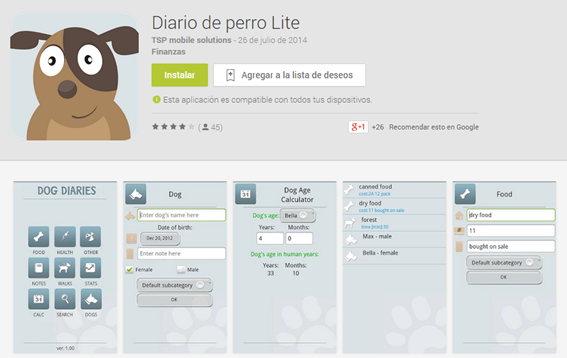
\includegraphics[width=0.9\textwidth]{antes.png}
  \caption{Captura desde google play}
  \label{fig:Captura desde google play}
\end{figure}

\section{Situaci\'on con el proyecto}


Una vez implementado se podrán registrar todo tipo de mascotas en una sola aplicación lo cual facilitara el acceso a la información sobre los animales domésticos, además de permitir llevar un control sobre las actividades panificadas, las que se realizaron,  llevar un control de cada cuándo se debe comprar alimentó para dicho animal, revisar los antecedentes médicos  de éste. Por otra parte compartir las actividades realizadas con la principal red social Facebook.

\chapter{Planificación  del proyecto}


\section{Programación del proyecto}

\newpage

\section{Carta Gantt}
\begin{figure}[!h]
  \centering
    \includegraphics[width=1.3\textwidth\ ,angle=270]{cartagantt.png}
  \caption{Diagrama de Gantt}
  \label{fig:Diagrama de Gantt}
\end{figure}

\chapter{Android}

\section{¿Que es Android?}
Android es un sistema operativo móvil que se basa en una versión modificada de Linux,
fue desarrollado originalmente por una empresa del mismo nombre, Android lnc.
A diferencia de los sistemas operativos móviles mencionados anteriormente Google Android se impulso al mercado de manera libre y gratuito. Con ello la mayor parte del
código de Android se encuentra bajo la licencia de código abierto Apache, lo que significa
que cualquier persona que quiera utilizar Android pueden hacerlo descargando el código
fuente. Por otra parte los proveedores de dispositivos móviles pueden añadir sus propias
ampliaciones de Android para brindar un producto que se pueda diferenciar de sus competidores. Este modelo simple de desarrollo Android lo hace muy atractivo y por ello ha
despertado el interés de muchos proveedores y desarrolladores de aplicaciones.
\section{Historia de Android}

\subsection{Android 1.6 Donut}
Toda la información del mundo a tu alcance: busca en la Web, obtén indicaciones… o simplemente mira videos de gatos.
\subsection{Android 2.0 Eclair}
Haz lo que quieras con tu pantalla principal. Organiza las aplicaciones y los widgets en varias pantallas y dentro de carpetas. Los increíbles fondos de pantalla animados responden al tacto.
\subsection{Android 2.2 Froyo}
Solo tienes que hablar para usar el Dictado por voz que te permite ingresar texto y las Acciones de voz que te dejan controlar el teléfono.
\subsection{Android 2.3 Gingerbread}
Los nuevos sensores hacen que Android sea excelente para juegos. Puedes tocar, presionar, inclinar y pasarte el día jugando.
\subsection{Android 3.0 Honeycomb}
Optimizada para tablets, esta versión abre nuevos horizontes donde quiera que estés.
\subsection{Android 4.0 Ice Cream Sandwich}
Android madura con un nuevo y refinado diseño. Sencillo, atractivo y más inteligente.
\subsection{Android 4.1 Jelly Bean}
Android es rápido y funciona a la perfección con gráficos definidos. Con Google Now, consigues la información que necesitas en el momento justo, con más de un millón de aplicaciones en Google Play y miles de dispositivos Android, tienes la libertad de hacer lo que quieras en el dispositivo que más te guste.
Mejoras:

\flushleft
\begin{itemize}
 \item Perfiles restringidos para tabletas: Ahora puede limitar el acceso a aplicaciones y contenido en el hogar y el trabajo.
 \item Soporte Bluetooth Smart: Bluetooth inteligente minimiza el uso de energía durante la medición y transmisión de datos de medidores de estado físico como Fitbit, Runtastic y otros dispositivos
 \item Autocompletado en  el discado telefónico:  Simplemente comienza a tocar los números o letras y el teclado de marcación sugerirá automáticamente los números o nombres.
\end{itemize}


\subsection{Android 4.4 KitKat}

Inteligente, simple y realmente tuyo. Diseño perfeccionado, rendimiento mejorado y nuevas funciones.
Mejoras:
\flushleft
\begin{itemize}

 \item Un diseño más pulido, un mejor rendimiento y nuevas características.
 \item Sólo decir ``OK Google": No es necesario tocar la pantalla para hacer las cosas. Cuando esta en la pantalla principal o en Google.  Ahora, puede decir ``OK Google" para iniciar la búsqueda de voz, enviar un texto, obtener direcciones o incluso reproducir una canción.
 \item Un trabajo de arte: Mientras se escucha música en su dispositivo, o el tiempo que proyecta películas de Chromecast, verá hermoso álbum de pantalla completa y el arte de la película, cuando el dispositivo está bloqueado. Puede reproducir, pausar, o buscar a un momento específico.
 \item Sumérgete: El nuevo modo de inmersión, que oculta automáticamente todo excepto lo que realmente quiere ver. Simplemente deslice el borde de la pantalla para traer de vuelta a sus barras de navegación y botones de estado.
 \item multitarea más rápido: Lleva el rendimiento del sistema a un nivel más alto mediante la optimización de la memoria y la mejora de su pantalla táctil para que responda más rápido y con mayor precisión que nunca.
 \item Inteligente y simple: Google inteligencia mejoran todos los rincones de la experiencia Android.
 \item Su oficina, en cualquier lugar: Crear y editar documentos, hojas de cálculo y presentaciones desde su teléfono o tableta con el nuevo diseño de Quickoffice.

\end{itemize}

\subsection{Android 5.0 Lollipop}

Ahora Android es mucho más tentador. Obtén la potencia de Android en pantallas grandes y pequeñas con la información que necesitas en el momento justo.
Mejoras:
\flushleft
\begin{itemize}
\item En más que su teléfono y la tableta: La potencia de Android en su reloj, su televisor e incluso su coche.
\item Continuar donde lo dejó: Las canciones, fotos, aplicaciones y búsquedas, incluso recientes de uno de sus dispositivos Android se pueden disfrutar inmediatamente a través de todos sus dispositivos Android.
\item Material desing: Movimiento fluido y con propósito.
\item Su dispositivo, sus reglas: Para un menor número de interrupciones y preocupaciones, ajusta la configuración para que sólo ciertas personas y notificaciones a superar.
\item Comparte tu dispositivo de forma segura con el modo de usuario invitado. O crear varias cuentas de usuario para permitir a los amigos que entrar en su dispositivo. En cualquier caso, nadie será capaz de acceder a cualquiera de sus cosas.
\item La energía para el largo plazo con una función de ahorro de batería que extiende su dispositivo por hasta 90 minutos. Y ahora es más fácil de administrar su consumo de energía - ver el tiempo estimado que queda antes de tener que cargar, y mientras se carga, aproximadamente la cantidad de tiempo hasta que se recargue  y esté  listo para funcionar.

\end{itemize}

\subsection{Android 6.0 Marshmallow}
Más para disfrutar
Mejoras:
\flushleft
\begin{itemize}

\item Los accesos directos más inteligentes para ir de un lugar a otro: Now on Tap anticipa lo que necesitas en cada momento. Con solo presionar, puedes obtener tarjetas con información útil y apps que satisfacen tu necesidad de conocer.
\item Una batería que funciona con mayor eficacia y no con mayor esfuerzo: Android Marshmallow ahorra energía para las acciones más importantes.
\item Mayor control para mayor tranquilidad: 
\item No es necesario que les otorgues acceso a las apps todo el tiempo. Android Marshmallow te permite determinar qué compartir y cuándo hacerlo. También puedes desactivar los permisos en el momento que quieras.
\item Evita las contraseñas complicadas. La clave está en tu mano. Desbloquea el teléfono con la huella digital y accede sin complicaciones a Play Store y a las apps de manera segura.
\end{itemize}

\section{Características}

Al ser una plataforma neutral de aplicaciones para dispositivos móviles, Android nodiferencia entre las aplicaciones básicas del dispositivo y las implementadas por los distintos
usuarios a la hora de establecer prioridades entre las aplicaciones. Esto hace posible que se puedan crear aplicaciones que sean tan importantes para el sistema operativo del teléfono
como las que vienen ya de serie.
Los background services (código que se ejecuta en un segundo plano) permiten la creación de aplicaciones que usan un modelo orientado a eventos, trabajando en silencio
cuando no se está manipulando el dispositivo o mientras se usan otras aplicaciones hasta que suena o vibra para llamar la atención. Android ofrece aplicaciones de mensajería P2P (peer-topeer) entre dispositivos para mejorar la comunicación.
En la siguiente lista se destacan algunas de las características más notables de la
plataforma Android (14):

\begin{enumerate}

\item Framework de aplicaciones permitiendo la reutilización y reemplazo de los
componentes. Se provee al usuario de numerosos servicios para ayudarle a desarrollar
aplicaciones.
\item Máquina virtual Dalvik optimizada para dispositivos móviles. Android posee su propia
máquina virtual para la gestión de las aplicaciones y su memoria.
\item Navegador integrado basado en el motor de código abierto WebKit, facilitando así el
acceso a Internet.
\item Gráficos optimizados mediante una biblioteca de gráficos 2D, los gráficos 3D están
basados en la especificación OpenGL ES 1.0 (aceleración de hardware opcional). Las
pantallas ayudan a esta mejora en los gráficos al ser cada vez más grandes, brillantes y
de alta resolución.
\item SQLite para almacenamiento de datos estructurados. Se proporciona una base de
datos relacional para cada aplicación mediante SQLite. Cada aplicación puede
beneficiarse del motor que la gestiona para almacenar los datos de forma segura y
eficiente.
\item Soporte multimedia para formatos comunes de audio, vídeo e imágenes planas
(MPEG4, H.264, MP3, AAC, AMR, JPG, PNG, GIF). Se dispone de una amplia colección
de bibliotecas que hacen posible dicho manejo multimedia.
\item Telefonía GSM (dependiendo del hardware).
\item Bluetooth, EDGE, 3G,4G LTE, Wi-Fi , NFC y Wi-Fi 5G(dependiendo del hardware). La conectividad a Internet
o entre distintos dispositivos depende del terminal que será el que determine los
distintos protocolos de comunicaciones que soporta.

\item Cámara, GPS o Glonas, brújula, lector de huellas y acelerómetro (dependiendo del hardware). Se incluyen
bibliotecas API que simplifican el desarrollo de aplicaciones involucrando el hardware
del dispositivo. Este cómodo acceso al hardware posibilita el hecho de no ser necesaria
la creación de una implementación específica en el software para cada diferente
dispositivo hardware.
\item Amplio entorno de desarrollo incluyendo un emulador del dispositivo, herramientas
para la depuración, perfiles de memoria y de rendimiento, En el IDE Android Studio.
\end{enumerate}


\section{Arquitectura Android}

 Android es una plataforma para dispositivos móviles que contiene una pila de software donde se incluye un sistema operativo, middleware y aplicaciones básicas para el usuario. 
 En las siguientes líneas se dará una visión global por capas de cuál es la arquitectura empleada en Android. Cada una de estas capas utiliza servicios ofrecidos por las anteriores, y ofrece a su vez los suyos propios a las capas de niveles superiores, tal como muestra la siguiente figura: 


\begin{figure}[h]
\begin{center}
    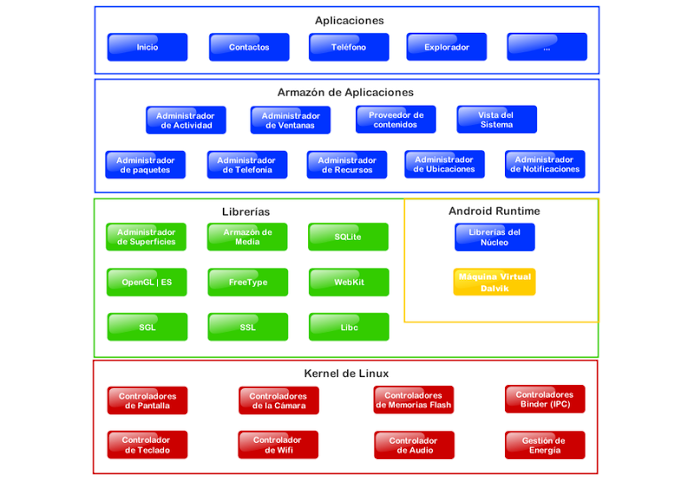
\includegraphics[width=1.1\textwidth\ ,angle=0]{arquitectura_android.png}
  \caption{Arquitectura de Android }
  \label{fig:Arquitectura de Android }
\end{center}
\end{figure}

\begin{itemize}




\item   \textbf{Aplicaciones:} Este nivel contiene, tanto las incluidas por defecto de Android como aquellas que el usuario vaya añadiendo posteriormente, ya sean de terceras empresas o de su propio desarrollo. Todas estas aplicaciones utilizan los servicios, las API y librerías de los niveles anteriores.

\item   \textbf{Framework de Aplicaciones:} Representa fundamentalmente el conjunto de herramientas de desarrollo de cualquier aplicación. Toda aplicación que se desarrolle para Android, ya sean las propias del dispositivo, las desarrolladas por Google o terceras compañías, o incluso las que el propio usuario cree, utilizan el mismo conjunto de API y el mismo ``framework", representado por este nivel.
        Entre las API más importantes ubicadas aquí, se pueden encontrar las siguientes:

\begin{itemize}

\item         \textbf{Activity Manager:} Conjunto de API que gestiona el ciclo de vida de las aplicaciones en Android.

\item      \textbf{ Window Manager:} Gestiona las ventanas de las aplicaciones y utiliza la librería Surface Manager.

\item   \textbf {Telephone Manager:} Incluye todas las API vinculadas a las funcionalidades propias del teléfono (llamadas, mensajes, etc.).

\item  \textbf {Content Provider:} Permite a cualquier aplicación compartir sus datos con las demás aplicaciones de Android. Por ejemplo, gracias a esta API la información de contactos, agenda, mensajes, etc. será accesible para otras aplicaciones.

\item    \textbf{ View System:} Proporciona un gran número de elementos para poder construir interfaces de usuario (GUI), como listas, mosaicos, botones, ``check-boxes", tamaño de ventanas, control de las interfaces mediante teclado, etc. Incluye también algunas vistas estándar para las funcionalidades más frecuentes.

\item      \textbf{ Location Manager:} Posibilita a las aplicaciones la obtención de información de localización y  posicionamiento.

\item    \textbf {Notification Manager:} Mediante el cual las aplicaciones, usando un mismo formato, comunican al usuario eventos que ocurran durante su ejecución: una llamada entrante, un mensaje recibido, conexión Wi-Fi disponible, ubicación en un punto determinado, etc. Si llevan asociada alguna acción, en Android denominada Intent, (por ejemplo, atender una llamada recibida) ésta se activa mediante un simple clic.
\item     \textbf { XMPP Service:} Colección de API para utilizar este protocolo de intercambio de mensajes basado en XML.

\end{itemize}

\item     \textbf {Librerías: }La siguiente capa se corresponde con las librerías utilizadas por Android. Éstas han sido escritas utilizando C/C++ y proporcionan a Android la mayor parte de sus capacidades más características. Junto al núcleo basado en Linux, estas librerías constituyen el corazón de Android.

              Entre las librerías más importantes ubicadas aquí, se pueden encontrar las siguientes:
\begin{itemize}

\item     \textbf  { Librería libc:} Incluye todas las cabeceras y funciones según el estándar del lenguaje C. Todas las demás librerías se definen en este lenguaje.

\item     \textbf { Librería Surface Manager:} Es la encargada de componer los diferentes elementos de navegación de pantalla. Gestiona también las ventanas pertenecientes a las distintas aplicaciones activas en cada momento.

\item     \textbf {  OpenGL/SL y SGL:} Representan las librerías gráficas y, por tanto, sustentan la capacidad gráfica de Android. OpenGL/SL maneja gráficos en 3D y permite utilizar, en caso de que esté disponible en el propio dispositivo móvil, el hardware encargado de proporcionar gráficos 3D. Por otro lado, SGL proporciona gráficos en 2D, por lo que será la librería más habitualmente utilizada por la mayoría de las aplicaciones. Una característica importante de la capacidad gráfica de Android es que es posible desarrollar aplicaciones que combinen gráficos en 3D y 2D.

\item     \textbf     {  Librería Media Libraries:} Proporciona todos los códecs necesarios para el contenido multimedia soportado en Android (vídeo, audio, imágenes estáticas y animadas, etc.)

\item     \textbf      { FreeType:} Permite trabajar de forma rápida  y sencilla con distintos tipos de fuentes.

\item     \textbf        { Librería SSL:} Posibilita la utilización de dicho protocolo para establecer comunicaciones seguras.

\item     \textbf         { Librería SQLite:} Creación y gestión de bases de datos relacionales. 

\item     \textbf     { Librería WebKit:} Proporciona un motor para las aplicaciones de tipo navegador y forma el núcleo del actual navegador incluido por defecto en la plataforma Android.
\end{itemize}
\end{itemize}

Tiempo de ejecución de Android: Al mismo nivel que las librerias de Android se sitúa el entorno de ejecución. Éste lo constituyen las Core Libraries, que son librerias con mulititud de clases Java y la máquina vistual Dalvik.
Núcleo Linux: Android utiliza el núcleo de Linux 2.6 como una capa de abstracción para el hardware disponible en los dispositivos móviles. Esta capa contiene los drivers necesarios para que cualquier componente hardware pueda ser utilizado mediante las llamadas correspondientes. Siempre que un fabricante incluye un nuevo elemento de hardware, lo primero que se debe realizar para que pueda ser utilizado desde Android es crear las librerias de control o drivers necesarios dentro de este kernel de Linux embebido en el propio Android.

\section{Runtime de Android}
Está basado en el concepto de máquina virtual utilizado en Java. Dado las
limitaciones de los dispositivos donde ha de ejecutarse Android (poca memoria y
procesador limitado) no fue posible utilizar una máquina virtual Java estándar.
Google tomó la decisión de crear una nueva, la máquina virtual Dalvik, que
respondiera mejor a estas limitaciones.
Algunas características de la máquina virtual Dalvik que facilitan esta
optimización de recursos son: que ejecuta ficheros Dalvik ejecutables (.dex) (formato
optimizado para ahorrar memoria). Además, está basada en registros. Cada
aplicación corre en su propio proceso Linux con su propia instancia de la máquina
virtual Dalvik. Delega al kernel de Linux algunas funciones como threading y el
manejo de la memoria a bajo nivel.
También se incluye en el Runtine de Android el “core libraries” con la mayoría
de las librerías disponibles en el lenguaje Java.

\begin{figure}[!ht]
  \centering
    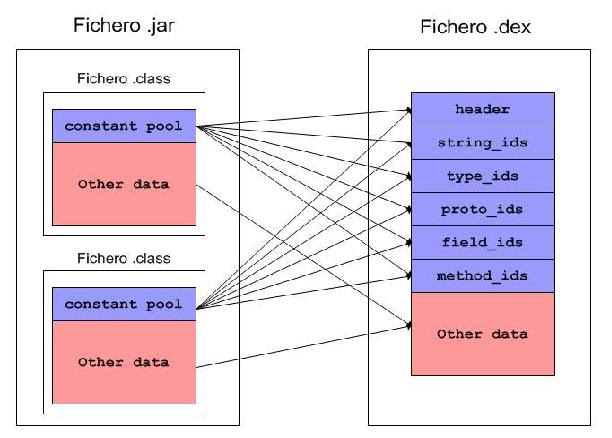
\includegraphics[width=1.1\textwidth\ ,angle=0]{ficheroDEX.JPG}
  \caption{Formato de un fichero .dex}
  \label{fig:Formato de un fichero .dex.}
\end{figure}

\section{Aplicaciones en Android}
Una aplicación Android corre dentro de su propio proceso Linux, por tanto, una característica fundamental de Android es que el tiempo y ciclo de vida de una aplicación no está controlado por la misma aplicación sino que lo determina el sistema a partir de una combinación de estados como pueden ser qué aplicaciones están funcionando, qué prioridad tienen para el usuario y cuánta memoria queda disponible en el sistema.

    Una aplicación en Android debe declarar todas sus actividades, los puntos de entrada, la comunicación, las capas, los permisos, y las intenciones a través de \textbf{AndroidManifest.xml}.  Es muy importante tener en consideración cómo estos componentes impactan en el tiempo de vida del proceso asociado con una aplicación, porque si no son empleados de manera apropiada, el sistema detendrá el proceso de la aplicación aún cuando se esté haciendo algo importante.

\subsection{Componentes}
\begin{itemize}
\item \textbf{Activity: }Sin duda es el componente más habitual de las aplicaciones para Android. Un componente Activity refleja una determinada actividad llevada a cabo por una aplicación, y que lleva asociada típicamente una ventana o interfaz de usuario; es importante señalar que no contempla únicamente el aspecto gráfico, sino que éste forma parte del componente Activity a través de vistas representadas por clases como View y sus derivadas. Este componente se implementa mediante la clase de mismo nombre Activity. La mayoría de las aplicaciones permiten la ejecución de varias acciones a través de la existencia de una o más pantallas. Por ejemplo, piénsese en una aplicación de mensajes de texto. En ella, la lista de contactos se muestra en una ventana. Mediante el despliegue de una segunda ventana, el usuario puede escribir el mensaje al contacto elegido, y en otra tercera puede repasar su historial de mensajes enviados o recibidos. Cada una de estas ventanas debería estar representada a través de un componente Activity, de forma que navegar de una ventana a otra implica lanzar una actividad o dormir otra. Android permite controlar por completo el \textbf{ciclo de vida} de los componentes Activity. 

     Tal y como se puede ver en el siguiente punto, una actividad tiene un ciclo de vida muy definido, que será igual para todas las actividades. Este ciclo de vida es impuesto por el SDK de Android. Las actividades tienen cuatro posibles estados: \textbf{Activa, pausada, parada y reiniciada. }
A la hora de diseñar una aplicación en Android hay que tener en cuenta su ciclo de vida.
Intent: Un Intent consiste básicamente en la voluntad de realizar alguna acción, generalmente asociada a unos datos. Lanzando un Intent, una aplicación puede delegar el trabajo en otra, de forma que el sistema se encarga de buscar qué aplicación de entre las instaladas, es la que puede llevar a cabo la acción solicitada. Por ejemplo, abrir una URL en algún navegador web, o escribir un correo electrónico desde algún cliente de correo. Los Intents están incluidos en el AndroidManifest porque describen dónde y cuándo puede comenzar una actividad. Cuando una actividad crea un Intent, éste puede tener descriptores de lo que se quiere hacer. Una vez se está ejecutando la aplicación, Android compara esta información del Intent con los Intents de cada aplicación, eligiendo el más adecuado para realizar la operación especificada por el llamante.
Broadcast Intent Receiver: Un componente Broadcast Intent Receiver se utiliza para lanzar alguna ejecución dentro de la aplicación actual cuando un determinado evento se produzca (generalmente, abrir un componente Activity). Por ejemplo, una llamada entrante o un SMS recibido. Este componente no tiene interfaz de usuario asociada, pero puede utilizar el API Notification Manager para avisar al usuario del evento producido a través de la barra de estado del dispositivo móvil. Este componente se implementa a través de una clase de nombre BroadcastReceiver. Para que Broadcast Intent Receiver funcione, no es necesario que la aplicación en cuestión sea la aplicación activa en el momento de producirse el evento. El sistema lanzará la aplicación si es necesario cuando el evento monotorizado tenga lugar.
\item \textbf{ Service: }Un componente Service representa una aplicación ejecutada sin interfaz de usuario, y que generalmente tiene lugar en segundo plano mientras otras aplicaciones (éstas con interfaz) son las que están activas en la pantalla del dispositivo. Un ejemplo típico de este componente es un reproductor de música. La interfaz del reproductor muestra al usuario las distintas canciones disponibles, así como los típicos botones de reproducción, pausa, volumen, etc. En el momento en el que el usuario reproduce una canción, ésta se escucha mientras se siguen visualizando todas las acciones anteriores, e incluso puede ejecutar una aplicación distinta sin que la música deje de sonar. La interfaz de usuario del reproductor sería un componente Activity, pero la música en reproducción sería un componente Service, porque se ejecuta en background. Este elemento está implementado por la clase de mismo nombre Service.
\item \textbf{Content Provider:} Con el componente Content Provider, cualquier aplicación en Android puede almacenar datos en un fichero, en una base de datos SQLite o en cualquier otro formato que considere. Además, estos datos pueden ser compartidos entre distintas aplicaciones. Una clase que implemente el componente Content Provider contendrá una serie de métodos que permiten almacenar, recuperar, actualizar y compartir los datos de una aplicación.

      Existe una colección de clases para distintos tipos de gestión de datos en el paquete android.provider. Además, cualquier formato adicional que se quiera implementar deberá pertenecer a este paquete y seguir sus estándares de funcionamiento.
    No todas las aplicaciones tienen que tener los cuatro componentes, pero cualquier aplicación será una combinación de estos.
\end{itemize}

\subsection {Estado de los procesos}
Como se ha mencionado anteriormente, cada aplicación de Android corre en su propio proceso, el cual es creado por la aplicación cuando se ejecuta y permanece hasta que la aplicación deja de trabajar o el sistema necesita memoria para otras aplicaciones. Android sitúa cada proceso en una jerarquía de "importancia" basada en estados, como se puede ver a continuación: 
\begin{itemize}
\item   \textbf{  Procesos en primer plano (Active process):} Es un proceso que aloja una Activity en la pantalla y con la que el usuario está interactuando (su método onResume() ha sido llamado) o que un IntentReceiver está ejecutándose. Este tipo de procesos serán eliminados como último recurso si el sistema necesitase memoria.
 
\item     \textbf{ Procesos visibles (Visible process):  }Es un proceso que aloja una Activity pero no está en primer plano (su método onPause() ha sido llamado). Esto ocurre en situaciones dónde la aplicación muestra un cuadro de diálogo para interactuar con el usuario. Este tipo de procesos no será eliminado en caso que sea necesaria la memoria para mantener a todos los procesos del primer plano corriendo.
 
\item   \textbf{    Procesos de servicio (Started service process):} Es un proceso que aloja un Service que ha sido iniciado con el método startService(). Este tipo de procesos no son visibles y suelen ser importantes para el usuario (conexión con servidores, reproducción de música).
 
\item     \textbf{ Procesos en segundo plano (Background process): }Es un proceso que aloja una Activity que no es actualmente visible para el usuario (su método onStop() ha sido llamado). Normalmente la eliminación de estos procesos no suponen un gran impacto para la actividad del usuario. Es muy usual que existan numerosos procesos de este tipo en el sistema, por lo que el sistema mantiene una lista para asegurar que el último proceso visto por el usuario sea el último en eliminarse en caso de necesitar memoria.
 
\item    \textbf{ Procesos vacíos (Empty process): }Es un proceso que no aloja ningún componente. La razón de existir de este proceso es tener una caché disponible de la aplicación para su próxima activación. Es común, que el sistema elimine este tipo de procesos con frecuencia para obtener memoria disponible.
 \end{itemize}
   Según esta jerarquía, Android prioriza los procesos existentes en el sistema y decide cuáles han de ser eliminados, con el fin de liberar recursos y poder lanzar la aplicación requerida.

\begin{figure}[!ht]
  \centering
    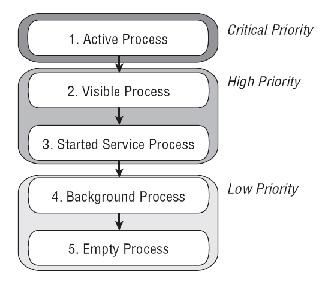
\includegraphics[width=1\textwidth\ ,angle=0]{procesosAndroid.jpg}
  \caption{Pila de prioridades.}
  \label{fig:Pila de prioridades. }
\end{figure}
  Para los procesos en segundo plano, existe una lista llamada \textbf{LRU }(Least Recently Used). En función de esta lista se van eliminando los procesos; los primeros que se eliminan son aquellos que llevan más tiempo sin usarse. Así el sistema se asegura de mantener vivos los procesos que se han usado recientemente.

\subsection{ Ciclo de vida de una actividad}
 El hecho de que cada aplicación se ejecuta en su propio proceso aporta beneficios en cuestiones básicas como seguridad, gestión de memoria, o la ocupación de la CPU del dispositivo móvil. Android se ocupa de lanzar y parar todos estos procesos, gestionar su ejecución y decidir qué hacer en función de los recursos disponibles y de las órdenes dadas por el usuario. 

   El usuario desconoce este comportamiento de Android. Simplemente es consciente de que mediante un simple clic pasa de una a otra aplicación y puede volver a cualquiera de ellas en el momento que lo desee. No debe preocuparse sobre cuál es la aplicación que realmente está activa, cuánta memoria está consumiendo, ni si existen o no recursos suficientes para abrir una aplicación adicional. Todo eso son tareas propias del sistema operativo. 

   Android lanza tantos procesos como permitan los recursos del dispositivo. Cada proceso, correspondiente a una aplicación, estará formado por una o varias actividades independientes (componentes Activity) de esa aplicación. Cuando el usuario navega de una actividad a otra, o abre una nueva aplicación, el sistema duerme dicho proceso y realiza una copia de su estado para poder recuperarlo más tarde. El proceso y la actividad siguen existiendo en el sistema, pero están dormidos y su estado ha sido guardado. Es entonces cuando crea, o despierta si ya existe, el proceso para la aplicación que debe ser lanzada, asumiendo que existan recursos para ello.
   Cada uno de los componentes básicos de Android tiene un ciclo de vida bien definido; esto implica que el desarrollador puede controlar en cada momento en qué estado se encuentra dicho componente, pudiendo así programar las acciones que mejor convengan. El componente \textbf{Activity}, probablemente el más importante, tiene un ciclo de vida como el mostrado en la siguiente figura.

\begin{figure}[!ht]
  \centering
    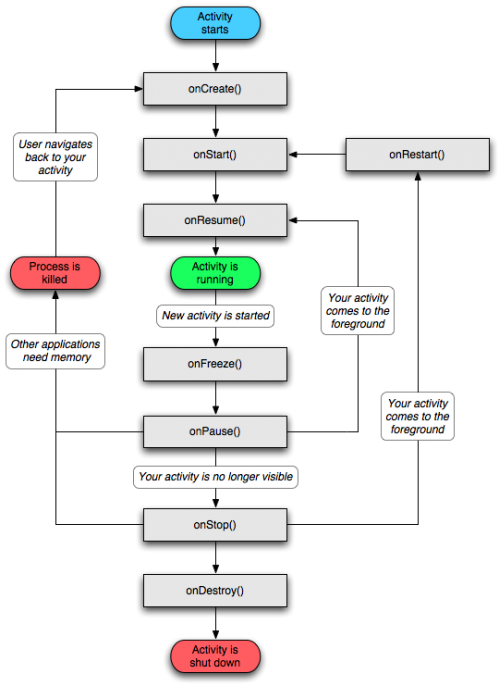
\includegraphics[width=0.6\textwidth\ ,angle=0]{activity_lifecycle.png}
  \caption{Ciclo de vida de una actividad.}
  \label{fig:Ciclo de vida de una actividad. }
\end{figure}



 De la figura anterior, pueden sacarse las siguientes conclusiones:
\begin{itemize}
\item onCreate(), onDestroy(): Abarcan todo el ciclo de vida. Cada uno de estos métodos representan el principio y el fin de la actividad.
\item onStart(), onStop():  Representan la parte visible del ciclo de vida. Desde onStart() hasta onStop(), la actividad será visible para el usuario, aunque es posible que no tenga el foco de acción por existir otras actividades superpuestas con las que el usuario está interactuando. Pueden ser llamados múltiples veces.
\item onResume(), onPause(): Delimitan la parte útil del ciclo de vida. Desde onResume() hasta onPause(), la actividad no sólo es visible, sino que además tiene el foco de la acción y el usuario puede interactuar con ella. 
   Tal y como se ve en el diagrama de la figura anterior, el proceso que mantiene a esta Activity puede ser eliminado cuando se encuentra en onPause() o en onStop(), es decir, cuando no tiene el foco de la aplicación. Android nunca elimina procesos con los que el usuario está interactuando en ese momento. Una vez se elimina el proceso, el usuario desconoce dicha situación y puede incluso volver atrás y querer usarlo de nuevo. Entonces el proceso se restaura gracias a una copia y vuelve a estar activo como si no hubiera sido eliminado. Además, la Activity puede haber estado en segundo plano, invisible, y entonces es despertada pasando por el estado onRestart(). 
\end{itemize}

   Pero, ¿qué ocurre en realidad cuando no existen recursos suficientes? Obviamente, los recursos son siempre limitados, más aun cuando se está hablando de dispositivos móviles. En el momento en el que Android detecta que no hay los recursos necesarios para poder lanzar una nueva aplicación, analiza los procesos existentes en ese momento y elimina los procesos que sean menos prioritarios para poder liberar sus recursos. 

   Cuando el usuario regresa a una actividad que está dormida, el sistema simplemente la despierta. En este caso, no es necesario recuperar el estado guardado porque el proceso todavía existe y mantiene el mismo estado. Sin embargo, cuando el usuario quiere regresar a una aplicación cuyo proceso ya no existe porque se necesitaba liberar sus recursos, Android lo crea de nuevo y utiliza el estado previamente guardado para poder restaurar una copia fresca del mismo. Como se ya ha explicado, el usuario no percibe esta situación ni conoce si el proceso ha sido eliminado o está dormido.

\chapter{Metodología Kanban}

Para este proyecto se decidió optar por la metodología Kanban ya que es muy fácil de utilizar, actualizar y asumir por parte del equipo. Además, destaca por ser una técnica de gestión de las tareas muy visual, que permite ver a golpe de vista el estado de los proyectos, así como también pautar el desarrollo del trabajo de manera efectiva.
Los principios de la metodología Kanban
La metodología Kanban se basa en una serie de principios que la diferencian del resto de metodologías conocidas como ágiles:
\flushleft
\begin{itemize}

\item Calidad garantizada. Todo lo que se hace debe salir bien a la primera, no hay margen de error. De aquí a que en Kanban no se premie la rapidez, sino la calidad final de las tareas realizadas. Esto se basa en el hecho que muchas veces cuesta más arreglarlo después que hacerlo bien a la primera.
\item Reducción del desperdicio. Kanban se basa en hacer solamente lo justo y necesario, pero hacerlo bien. Esto supone la reducción de todo aquello que es superficial o secundario (principio YAGNI).
\item Mejora continua. Kanban no es simplemente un método de gestión, sino también un sistema de mejora en el desarrollo de proyectos, según los objetivos a alcanzar.
\item Flexibilidad. Lo siguiente a realizar se decide del backlog (o tareas pendientes acumuladas), pudiéndose priorizar aquellas tareas entrantes según las necesidades del momento (capacidad de dar respuesta a tareas imprevistas). 
\end{itemize}
\section{Herramientas de desarrollo de software}
\begin{itemize}
\item \textbf{Android Studio:}es un entorno de desarrollo integrado oficial para aplicaciones móviles del sistema operativo Android,es compatible con los sistemas operativos Windows, MacOS y GNU/Linux.
\item \textbf{WampServer:} es un entrono de desarrollo web para Wiondows con el que es posible crear aplicaciones web con Apache,Php y bases de datos MySQL.
\item \textbf{ProjetLibre:} es el software de administración y gestión de proyectos de código abierto que continúa la trayectoria iniciada por la antigua y reconocida herramienta Openproj. Basado en el lenguaje de programación Java, es compatible con los sistemas operativos Windows, MacOS y GNU/Linux.
\item \textbf{Texmaker:}es un editor gratuito distribuido bajo la licencia GPL para escribir documentos de texto, multiplataforma, que integra muchas herramientas necesarias para desarrollar documentos con LaTeX, en una sola aplicación. 
\end{itemize}


\section{Herramientas de desarrollo de material visual}
\begin{itemize}
\item \textbf{Metro Studio:} es una colección de mas de 6.000 plantillas de iconos, fáciles de personalizar para crea cientos de iconos. 
\end{itemize}

\section{Hardware}

Para llevar acabo este proyecto se cuenta con un computador portátil.

Notebook HP DV6 7380LA.\\

CPU: Intel Core I7 3630QM.\\

GPU: Nvidia Geforce GT 650M.\\

RAM: 16 GB.\\

SDD: 256 GB.\\

Sistema Operativo: Windows 7 Ultimate x64.\\



\chapter{Proyecto}
\section{Analisis}
\newpage
\subsection{Requerimientos funcionales}

los requerimientos funcionales son los definidos en \ref{tabla:Tabla de Requerimientos.}
%\begin{enumerate}
%\item{enumerate}
%\item{enumerate}
%\end{enumerate}
%\subsection{Requerimientos No funcionales}
%\begin{enumerate}
%\item
%\item
%\end{enumerate}

\begin{table}[htb]
\begin{center}
\begin{tabular}{|l|l|p{5cm}|} 

\hline
Módulos principales & Funcionalidad
requerida & Funcionalidad objetiva \\
\hline \hline  \hline 
\multirow{3}{2cm}{Login} 
&Crear cuenta & Registrar un usuario nuevo \\ \cline{2-3}
&Ingresar  & Ingresar la aplicación\\ \cline{2-3}
&Recuperar la contraseña &  \\ \cline{1-3}

\multirow{6}{2cm}{Actividades} 
& Flitrar actividades& Filtrar actividades por mascota,  tipo de actividad, etc. \\ \cline{2-3}
&Ver actividad  & Ver los detalles de la actividad.\\ \cline{2-3}
&Eliminar actividad &  Elimina una o varias actividades . \\ \cline{2-3}
&Ver mascota  & Ver los detalles de una mascota.\\ \cline{2-3}
&Ver gastos  & Ver el resumen de los gastos.\\ \cline{2-3}
&Agregar actividad & Agrega una actividad para determinada mascota.  \\ \cline{1-3}

\multirow{2}{2cm}{Mascota} 
& Editar & Permite editar los datos de la mascota. \\ \cline{2-3}
& Eliminar  & Permitir eliminar una Mascota.\\ \cline{1-3}

\multirow{2}{2cm}{Actividad}
& Editar& Editar los detalles de la actividad. \\ \cline{2-3}
& Eliminar  & Elimina una determinada actividad \\ \cline{1-3}

\multirow{3}{2cm}{Costos}
 & Ver un grafico  & Ver un grafico con la el gasto de los utimos 12 meses en pesos .\\ \cline{2-3}
& Datelle de los gastos &Ver el detalle de los gastos realizados el ultimo mes en pesos.\\ \cline{1-3}

\end{tabular}
\caption{Tabla de Requerimientos.}
\label{tabla:Tabla de Requerimientos.}
\end{center}
\end{table}

\newpage
\subsection{Requerimientos no funcionales}
A continuación se detallarán los requisitos no funcionales.

\begin{itemize}
\item La aplicación funcionara para la version 4.0 de Android en adelante.
\item Los motores de base de dato SQL lite y MySQL.
\item La aplicación debe ser facil de usar.
\item  El dispositivo debe tener conexión a internet para recuperar la contraseña .
\item
\item
\item
\end{itemize}
\subsection{Casos de uso}
Mediante el diagrama de casos de uso mostraremos de una forma gráfica la
funcionalidad de todo el sistema y como el usuario de la aplicación (Actor) interacciona
con el mismo.

\section{Dise\~no}
\subsection{Clases}
\begin{enumerate}
\item a
\item a
\end{enumerate}
\subsection{interfaz}

\subsection{Pantallas}
\begin{enumerate}
\item a\item a
\item a
\end{enumerate}
\section{Implementacion}
\subsection{Arquitectura}








\chapter{Conclusiones y Trabajo Futuro}
\subsection{Conclusiones}
\subsection{Trabajo Futuro}

\bibliographystyle{these}
%Usar bibliografia con bibtex.
%\bibliography{biblio}

\appendix
\renewcommand{\appendixname}{Anexo N}

\chapter{Anexo N}


\end{document}
